% !TEX root = ../main.tex
\section{\emph{Local} component}\label{sec:local-component}

\begin{figure}[htbp]
\centering
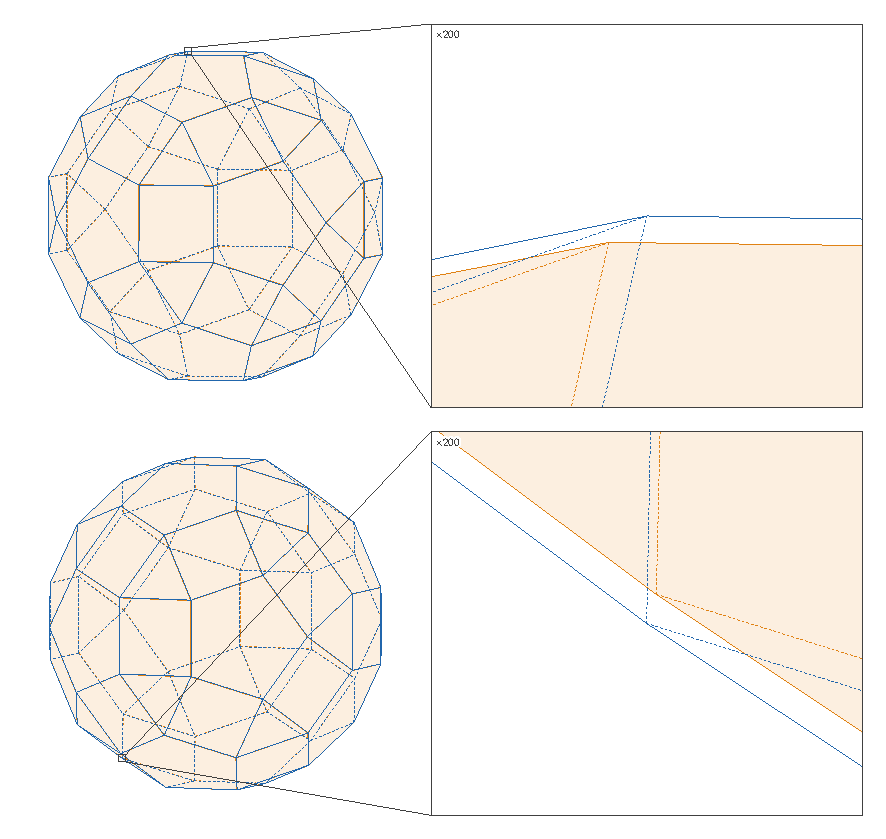
\includegraphics[width=\linewidth]{figures/local}
\caption{Two configurations near aligned ones, in the regions of Local covers: $[1/4,1/20,(1/1000,1/2000,-1/1000)]$ and $[2/5,1/10,(-1/1000,1/1000,1/2000)]$. The \fc{Hole}{hole (orange)} and the \fc{Plug}{plug (blue)} as in \cref{fig:global-examples}. The two shadows almost coincide; the enlargements, $200$ times, show a projected plug vertex protruding beyond the hole's shadow by about $0.004$, the outward motion that the face zooms certify for every small rotation.}
\label{fig:local-examples}
\end{figure}

At an aligned configuration, the plug and hole coincide. A small relative
rotation can nevertheless make a projected plug vertex protrude beyond
the hole's shadow.
The \emph{Local} component uses this outward motion to eliminate whole
neighbourhoods containing aligned configurations, extending the Global component, which
cannot eliminate any box containing an aligned configuration, as established in
\cref{subsec:range-and-insufficiency-for-touch-configurations}.

\subsection{Geometry of \emph{aligned} configurations}\label{subsec:geometry-of-aligned-configurations}

Use the representative $\mathbf r=\mathbf0$ for alignment, so the plug
initially has the hole's orientation. Fix the viewing parameters $(s,t)$
and rotate the plug about a fixed axis through the origin. A vertex
off the axis moves on a circle; its orthogonal projection traces an
ellipse, possibly reduced to a line segment. A vertex on the axis stays
fixed. The rational screen map preserves these descriptions, since it
is an invertible linear change of coordinates on the projection plane.

Choose a vertex whose initial projection lies on a supporting line of
the hole shadow. If its projection moves beyond that line, away from the
hole shadow, the plug cannot fit. We seek a positive interval of rotation
throughout which this protrusion persists, starting immediately after zero rotation.
An outward initial velocity can establish the direction of motion, but
the curvature of the trajectory also matters when determining how far
the plug can rotate before the vertex returns to the supporting line.

For a five-dimensional neighbourhood, this conclusion must hold uniformly
as both $(s,t)$ and the rotation axis vary. Different axes may require
different vertices and supporting lines. We therefore use a finite family
of such choices, each valid throughout a specified region of viewing
parameters and rotation directions. Together they must account for every
direction of rotation and give a common positive bound on its magnitude.
When these bounds hold, they certify that the neighbourhood contains no
fit configurations:
zero-rotation configurations remain touch configurations, while every
nonzero rotation within the bound yields a poke configuration.


\subsection{Eliminating \emph{aligned} configurations}\label{subsec:eliminating-aligned-configurations}

For a nonzero rotation vector $\mathbf r=(r_1,r_2,r_3)$, separate its magnitude
and direction by writing
\begin{equation}\label{eq:normalised-rotation-direction}
  \delta=\lVert\mathbf r\rVert_\infty
         :=\max\{|r_1|,|r_2|,|r_3|\}>0,
  \qquad \widehat{\mathbf r}=\frac{\mathbf r}{\delta},
  \qquad \mathbf r=\delta\widehat{\mathbf r}.
\end{equation}
The normalised vector lies on the boundary of the cube ${[-1,1]}^3$.
We denote its six closed faces by
\[
  F_i^\sigma=\{\widehat{\mathbf r}\in{[-1,1]}^3:
                     \widehat r_i=\sigma\},
  \qquad i\in\{1,2,3\},\quad\sigma\in\{-1,1\}.
\]
On $F_i^\sigma$, coordinate $i$ is fixed at $\sigma$, and the other
two belong to $[-1,1]$.
When several coordinates have maximum absolute value, the vector belongs
to several faces, so the six faces together contain every direction.
The two free face coordinates and $\delta$ describe the three rotational
degrees of freedom.

We use the maximum norm because its unit sphere is made of six squares:
the rotation directions on one face form a box, which is where the
Bernstein sign test works, and a bound on $\delta$ bounds all three
rotation coordinates directly. Here $\widehat{\mathbf r}$ need not have
Euclidean length one, and $\delta$ is not the rotation angle. By
\cref{eq:relative-rotation}, the unit axis and angle are respectively
\[
  \frac{\widehat{\mathbf r}}{\lVert\widehat{\mathbf r}\rVert},
  \qquad
  \theta=2\arctan\bigl(\delta\lVert\widehat{\mathbf r}\rVert\bigr).
\]

\paragraph{Supporting lines throughout a viewing region.}
Fix a closed axis-parallel rectangle $W\subseteq\mathbb R^2$ of viewing
parameters $(s,t)$.
Select a hole vertex $\mathbf v\in V$ and a normal $\mathbf n(s,t)$ perpendicular
to $\mathbf u=(s,t,1)$. For every $(s,t)\in W$,
the projection of $\mathbf v$ must lie on a supporting line of the hole
shadow with outward normal $\mathbf n(s,t)$:
\begin{equation}\label{eq:local-support-conditions}
  \mathbf n(s,t)\cdot(\mathbf w-\mathbf v)\le0
  \qquad\text{for all }\mathbf w\in V.
\end{equation}
As in the Global component, equalities are allowed. Since $\mathbf n\perp\mathbf u$,
the same inequalities compare the orthogonal projections onto the screen.
As the plug rotates, the projection of the vertex starting at $\mathbf v$
protrudes beyond the hole shadow as soon as
$\mathbf n\cdot(R_P(\mathbf r)\mathbf v-\mathbf v)>0$.

The normal must stay perpendicular to $\mathbf u$ as $(s,t)$ varies. We use
either the moving direction \cref{eq:moving-support-direction} of the
Global component, or the direction
\begin{equation}\label{eq:local-fixed-screen-direction}
  \mathbf n(s,t)=(n_1,n_2,-sn_1-tn_2),
  \qquad n_1,n_2\in\mathbb Q(\sqrt5),\quad(n_1,n_2)\ne(0,0),
\end{equation}
which corresponds to the fixed planar support direction $(n_1,n_2)$ in the
screen coordinates $L_{s,t}$ of \cref{eq:screen-map}. For either form, each
of the sixty inequalities in \cref{eq:local-support-conditions} is affine
in $(s,t)$, so checking them at the four corners of $W$ establishes
support throughout $W$.

\paragraph{Displacement under rotation.}
To determine how long this protrusion persists,
we need both its initial direction of motion and the bending of its
circular trajectory. For a vertex off the rotation axis,
$\widehat{\mathbf r}\times\mathbf v$ points along the initial tangent,
while $\widehat{\mathbf r}\times(\widehat{\mathbf r}\times\mathbf v)$
points towards the axis. Taking their components along the outward
normal gives the two displacement polynomials
\begin{equation}\label{eq:local-displacement-polynomials}
  p_1=\mathbf n\cdot(\widehat{\mathbf r}\times\mathbf v),
  \qquad
  p_2=\mathbf n\cdot
       \bigl(\widehat{\mathbf r}\times
                    (\widehat{\mathbf r}\times\mathbf v)\bigr).
\end{equation}
Their variables are $s,t$ and the two free coordinates of
$\widehat{\mathbf r}$ on $F_i^\sigma$. A positive $p_1$ indicates
initial outward motion, whereas a negative $p_2$ opposes it as the
rotation grows. Subtracting $\mathbf v$ from
\cref{eq:relative-rotation}, substituting
$\mathbf r=\delta\widehat{\mathbf r}$, and using
\[
  \widehat{\mathbf r}\times
    (\widehat{\mathbf r}\times\mathbf v)
  =\widehat{\mathbf r}(\widehat{\mathbf r}\cdot\mathbf v)
     -\lVert\widehat{\mathbf r}\rVert^2\mathbf v
\]
gives the exact identity
\begin{equation}\label{eq:local-radial-displacement}
  \mathbf n\cdot
    \bigl(R_P(\delta\widehat{\mathbf r})\mathbf v-\mathbf v\bigr)
   =\frac{2\delta}
          {1+\delta^2\lVert\widehat{\mathbf r}\rVert^2}
       (p_1+\delta p_2).
\end{equation}

\paragraph{Dividing out the size of the rotation.}
Both sides of \cref{eq:local-radial-displacement} vanish at $\delta=0$,
where the configuration is aligned. This is why no box containing an
aligned configuration can be eliminated by testing the displacement
directly: its sign is zero there, and the Bernstein sign test must refuse
it. The factor $\delta$, however, is explicit. In terms of the gap
polynomial \cref{eq:support-gap-polynomial} of the Global component,
with the plug vertex $\mathbf v_p=\mathbf v$ and the rotation denominator
$d=1+\delta^2\lVert\widehat{\mathbf r}\rVert^2$, the identity reads
\begin{equation}\label{eq:local-gap-factorisation}
  p_{\mathbf v}
   =\mathbf n\cdot\bigl(\widehat R_P(\delta\widehat{\mathbf r})\mathbf v-d\mathbf v\bigr)
   =2\delta\,(p_1+\delta p_2),
\end{equation}
an identity of polynomials in $s$, $t$, $\delta$ and the two free
coordinates of $\widehat{\mathbf r}$. If the quotient $2(p_1+\delta p_2)$
is positive throughout a closed region of these five variables with
$0\le\delta\le\delta_{\max}$, then the vertex protrudes at every
positive $\delta$ in the region, and the configurations with $\delta=0$ are
aligned touch configurations, which are not fits. The Bernstein sign test
can certify the quotient directly, and it can succeed even at $\delta=0$,
where the quotient is $2p_1$: it only needs outward initial motion.

This observation is the idea behind every remaining component of the
proof. Near a set of configurations that are already known not to be fits,
we change coordinates so that some coordinates measure the distance from
that set, divide a necessary inequality exactly by a power of those
distances, and certify the quotient with Bernstein coefficients.

\subsection{The zoom lemma}\label{subsec:the-zoom-lemma}

The rest of the proof uses the same step with other sets in place of the
aligned configurations and other distances in place of $\delta$. We
therefore state it once, in a form that covers every use.

Several of the coordinate changes below scale the viewing direction, so we
allow the viewing vector to be any positive multiple of $(s,t,1)$: a vector
$\mathbf u$ with $u_3>0$ and a rotation vector $\mathbf r$ describe the
configuration $[u_1/u_3,u_2/u_3,\mathbf r]$.

\begin{definition}[No-fit sets and witnesses]\label{def:witness}
  A \emph{no-fit set} is a set of configurations containing no fit.
  A \emph{witness} is a polynomial $p$ in $\mathbf u$ and $\mathbf r$,
  homogeneous in $\mathbf u$, together with finitely many linear forms
  $\lambda_1,\dots,\lambda_m$ in $\mathbf u$, possibly none, its
  \emph{validity conditions}, such that $p\le0$ at every fit in $D$
  whose viewing vector satisfies $\lambda_j(\mathbf u)\ge0$ for all $j$.
\end{definition}

By homogeneity, the signs of $p$ and of each $\lambda_j$ do not depend on
the positive multiple chosen for $\mathbf u$. The aligned configurations form
a no-fit set: by \cref{eq:relative-rotation}, $\mathbf r=\mathbf0$ gives
$P_c=H_c$, and a compact shadow never lies in its own interior. Two kinds
of witnesses suffice for the whole proof.
\begin{itemize}
  \item A gap polynomial \cref{eq:support-gap-polynomial}, with
    $\mathbf n$ written as a linear function of $\mathbf u$ (for
    \cref{eq:local-fixed-screen-direction}, as
    $(u_3n_1,u_3n_2,-u_1n_1-u_2n_2)$), whose validity conditions are the
    support inequalities \cref{eq:local-support-conditions} of its hole
    vertex $\mathbf v$. Where they hold, the projection of $\mathbf v$ lies on
    a supporting line of the hole shadow with outward normal $\mathbf n$; a fit
    puts the projected plug vertex in the interior of the hole shadow, strictly
    on the inner side of that line, so the gap polynomial is negative there.
  \item A \emph{domain polynomial}: the polynomial $q$ of an inequality
    $q\le0$ defining $D$, written homogeneously in $\mathbf u$ (the fold
    inequality, for example, as ${\ell_g}^2-\lVert\mathbf u\rVert^2$), without
    validity conditions. It is nonpositive on all of $D$.
\end{itemize}

\begin{definition}[Zooms]\label{def:zoom}
  A \emph{zoom} is a polynomial map $\mathcal Z$ from a box $Y$ of
  \emph{zoom coordinates} $\mathbf y=(y_1,\dots,y_5)$ to viewing and
  rotation vectors, $\mathcal Z(\mathbf y)=(\mathbf u(\mathbf y),\mathbf r(\mathbf y))$,
  together with a set of designated \emph{distance coordinates}, such that
  \begin{enumerate}
    \item $u_3(\mathbf y)>0$ on $Y$, and each component of
      $\mathbf u(\mathbf y)$ has degree at most one in each zoom coordinate;
    \item each distance coordinate is nonnegative on $Y$, and wherever one
      of them vanishes, $\mathcal Z(\mathbf y)$ lies in a fixed no-fit set,
      the zoom's no-fit set.
  \end{enumerate}
  A monomial $\mathbf y^{\mathbf a}=\prod_jy_j^{a_j}$ in the distance
  coordinates is a \emph{zoom factor}, and a closed box $C\subseteq Y$ is a
  \emph{zoom cell}.
\end{definition}

The name describes what a zoom does near its no-fit set. A distance
coordinate measures how far a configuration is from that set, and the
other coordinates describe the direction of departure in units of that
distance. A thin neighbourhood of the no-fit set is thereby spread out
over a whole box, much as a camera zooms in on a detail, and once the zoom
factor is divided out, the behaviour of a witness arbitrarily close to the
no-fit set becomes the behaviour of a polynomial on a box, where Bernstein
coefficients can see it. The degree condition in the first requirement is
what allows validity conditions to be checked at the corners of a cell.

\begin{lemma}[Zoom lemma]\label{lem:zoom-lemma}
  Let $\mathcal Z$ be a zoom, $C$ a zoom cell and $p$ a witness. Suppose that
  \begin{enumerate}
    \item $p(\mathcal Z(\mathbf y))=\mathbf y^{\mathbf a}N(\mathbf y)$ exactly,
      as polynomials, for a zoom factor $\mathbf y^{\mathbf a}$;
    \item every validity condition of $p$ holds at the viewing vectors
      $\mathbf u(\mathbf y)$ of the corners $\mathbf y$ of $C$;
    \item every tensor Bernstein coefficient of $N$ on $C$ is strictly
      positive.
  \end{enumerate}
  Then no configuration $\mathcal Z(\mathbf y)$ with $\mathbf y\in C$ is a
  fit lying in $D$. More precisely, each such configuration lies in the
  zoom's no-fit set or satisfies $p>0$ and the validity conditions of $p$;
  for a gap polynomial, the latter makes it a poke configuration.
\end{lemma}
\begin{proof}
  By \cref{lem:bernstein-sign-test} applied to $-N$, we have $N>0$
  throughout $C$. Let $\mathbf y\in C$. If a distance coordinate with
  $a_j>0$ vanishes at $\mathbf y$, then $\mathcal Z(\mathbf y)$ lies in the
  no-fit set. Otherwise $\mathbf y^{\mathbf a}>0$, so
  $p(\mathcal Z(\mathbf y))>0$, and by homogeneity $p>0$ at the
  configuration itself. Each validity condition $\lambda_j(\mathbf u(\mathbf y))$
  is linear in $\mathbf u$, and $\mathbf u(\mathbf y)$ has degree at most one
  in each zoom coordinate, so the condition is affine in each coordinate
  separately; varying one coordinate at a time, its minimum over $C$ is
  attained at a corner. The validity conditions therefore hold throughout
  $C$, and since $p$ is a witness, $p>0$ excludes a fit in $D$. For a gap
  polynomial, $p>0$ places the projected plug vertex strictly beyond a
  supporting line of the hole shadow.
\end{proof}

The lemma separates what is proved by hand from what is checked by the
computer. By hand: that a set is a no-fit set, that a polynomial is a
witness, and that the zooms reach every configuration of the region
concerned. By exact computation, cell by cell: the division, the validity
conditions at the corners and the signs of the Bernstein coefficients.
The division must be exact; a single term that is not a multiple of the
zoom factor means the cell is refused.

The tests of the preceding components are the simplest case, with nothing
divided out. With the identity map on a search box as the zoom, no distance
coordinates and the zoom factor one, the lemma for a domain polynomial is
exactly the test of the Domain component. The test of the Global component
is the same idea for gap polynomials, except that instead of checking the
validity conditions of one hole vertex at the corners, it requires the gap
polynomials of all sixty hole vertices to be positive, so that whichever
hole vertex supports the shadow, its gap polynomial is positive.

\paragraph{Tube zooms.}
The zooms of this paper are of two kinds. Both use coordinates adapted to a
no-fit set: after an invertible affine change of variables, the
\emph{base} coordinates $\mathbf z_b$ run along the no-fit set and the
\emph{offset} coordinates $\mathbf z_o$ measure the displacement away from
it, so that the configurations with $\mathbf z_o=\mathbf0$ lie in the no-fit
set. As for the rotation vector above, the offsets are normalised on the
faces of a box. Let $\Phi\subseteq{[-1,1]}^m$ be a box whose every side is
$[-1,0]$, $[0,1]$ or $[-1,1]$; a side $[0,1]$ or $[-1,0]$ records that an
offset coordinate has a fixed sign. The \emph{cone} of $\Phi$ is the set of
vectors whose coordinates have the signs that $\Phi$ allows: nonnegative
where its side is $[0,1]$, nonpositive where it is $[-1,0]$. For
$\mathbf z\ne\mathbf0$ in the cone, $\mathbf z/\lVert\mathbf z\rVert_\infty$
lies on a \emph{face} of $\Phi$, a side where one coordinate equals $\pm1$.

Let the base coordinates range over a box $\Sigma_b$, and let
$\delta_{\max}>0$. For each face $F$ of $\Phi$, the \emph{tube zoom}
$\mathcal T_F$ has as zoom coordinates the base coordinates
$\mathbf z_b\in\Sigma_b$, the distance coordinate $\delta\in[0,\delta_{\max}]$
and the free coordinates of $\widehat{\mathbf f}\in F$, and it sets
$\mathbf z_o=\delta\widehat{\mathbf f}$. The \emph{covered set} of the
family is
\begin{equation}\label{eq:tube-covered-set}
  \{(\mathbf z_b,\mathbf z_o):\ \mathbf z_b\in\Sigma_b,\ \mathbf z_o\in\delta_{\max}\Phi\}.
\end{equation}

\begin{lemma}[Tube coverage]\label{lem:tube-coverage}
  Every configuration in the covered set of a family of tube zooms lies in
  the no-fit set or is the image of a point in the domain of one of them.
\end{lemma}
\begin{proof}
  Let $\delta=\lVert\mathbf z_o\rVert_\infty\le\delta_{\max}$. If $\delta=0$, the
  configuration lies in the no-fit set. Otherwise
  $\widehat{\mathbf f}=\mathbf z_o/\delta$ lies on a face $F$ of $\Phi$, and
  $(\mathbf z_b,\delta,\widehat{\mathbf f})$ is a point of the domain of
  $\mathcal T_F$.
\end{proof}

Tube zooms divide out one distance, the size of the offset. They are used
around the aligned configurations below and along two families of
non-aligned touch configurations in \cref{sec:arc-configurations}. At a few
special points, one distance is not enough, and
\cref{sec:square-and-pentagon-configurations} introduces \emph{point zooms},
which divide out two: the distance along the no-fit set from the special
point, and the offset measured relative to it. Where two families of touch
configurations cross, \cref{sec:endpoint-and-crossing-configurations} adds
a \emph{hand-over} from zooms around one family to zooms around the other.

\paragraph{Zoom covers.}
The cells of a family of zooms are found by subdivision. The domain of
each zoom is bisected in one coordinate at a time, keeping both children,
until every terminal cell carries a witness and a zoom factor satisfying
the hypotheses of \cref{lem:zoom-lemma}. The union of the children is their
parent, so by induction the terminal cells cover the domain. A family of
zooms with such subdivisions and witnesses is a \emph{zoom cover}; its
covered set is the covered set of its family. The cells and witnesses are
found by the program's generator (\texttt{rid generate}), but every cell is checked exactly before use,
so how they were found does not matter.

\subsection{Face zooms and the \emph{Local} component}\label{subsec:face-zooms-and-the-local-component}

The \emph{face zooms} are the tube zooms around the aligned
configurations. Their base coordinates are the viewing parameters
$(s,t)\in W$, their offset is the rotation vector $\mathbf r$ with
$\Phi={[-1,1]}^3$, whose six faces are the $F_i^\sigma$, and
\[
  \mathbf u=(s,t,1),\qquad \mathbf r=\delta\widehat{\mathbf r},
  \qquad \widehat{\mathbf r}\in F_i^\sigma,\quad 0\le\delta\le\delta_{\max}.
\]
Where the distance coordinate $\delta$ vanishes, $\mathbf r=\mathbf0$ and the
configuration is aligned. By \cref{eq:local-gap-factorisation}, a gap
polynomial whose plug vertex is its hole vertex is divisible by the zoom
factor $\delta$. The same holds for any plug vertex $\mathbf v_p$ whose
unrotated projection lies on the same supporting line throughout the cell,
for example the other end of a hole edge along it, since the gap then
vanishes at $\delta=0$; the exact division checks this. The covered set of
the six face zooms is the region
\begin{equation}\label{eq:local-region}
  W\times{[-\delta_{\max},\delta_{\max}]}^3 .
\end{equation}

\begin{proposition}[Soundness of the \emph{Local} component]\label{prop:soundness-of-the-local-component}
  Suppose a zoom cover of face zooms with covered set \cref{eq:local-region}
  has been checked, with a gap polynomial and a zoom factor $\delta$ or $1$ in
  every cell. Then every configuration in that region is a touch
  configuration when $\mathbf r=\mathbf0$ and a poke configuration
  otherwise. Any search box contained in the region can therefore be
  eliminated.
\end{proposition}
\begin{proof}
  By \cref{lem:tube-coverage}, a configuration of the region with
  $\mathbf r\ne\mathbf0$ is the image of a point of some face zoom's domain,
  and a terminal cell contains this point. By \cref{lem:zoom-lemma}, the
  cell's witness is positive there, so a projected plug vertex lies strictly
  beyond a supporting line of the hole shadow and the configuration is a
  poke configuration. Zero rotation yields an aligned and therefore touch
  configuration.
\end{proof}

\paragraph{Checking a search box.}
The Local component has a finite list of viewing rectangles $W$ with
checked zoom covers and bounds $\delta_{\max}$. It accepts a search box that
lies in one of the regions \cref{eq:local-region}: the product of its two
viewing intervals must lie in $W$, and each of its three rotation intervals
in $[-\delta_{\max},\delta_{\max}]$. Its certificate record names the
region, so that these endpoint comparisons can be repeated. The covers are
checked once, before the search; the test for a box is only this
inclusion. \Cref{fig:local-refinement} shows the effect of adding the Local
component.

\begin{figure}[htbp]
\centering
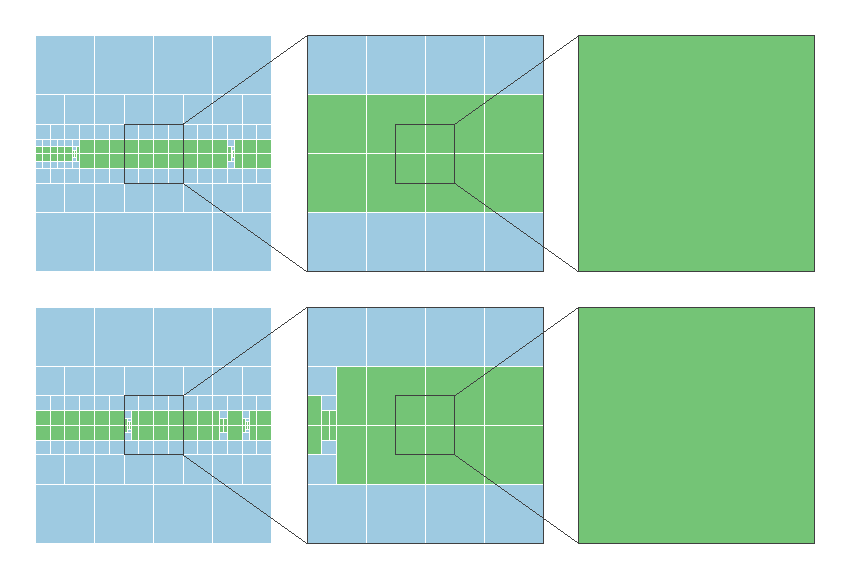
\includegraphics[width=\linewidth]{figures/local-refinement}
\caption{The slices of \cref{fig:global-refinement} with the \fc{Local}{Local component added (green)}. The unresolved band is gone: near the aligned configurations every piece lies in the region of a Local cover, and in the smallest window the whole window does at once.}
\label{fig:local-refinement}
\end{figure}

\subsection{Range and exotic viewing directions}\label{subsec:range-and-exotic-viewing-directions}

The Local component has 30 zoom covers of this kind, with bounds
$\delta_{\max}$ between $1/200$ and $1/20$ and 833 terminal cells in all.
Their viewing rectangles come from 30 rectangles with disjoint interiors,
each enlarged by $1/1024$ on every side (and cut to the viewing rectangle
$[0,2/3]\times[0,2/5]$ of $B_0$), so that neighbouring rectangles overlap and
a small search box on the boundary between two of them lies inside one.
For example, one of the regions is
\[
  \left[\frac16-\frac1{1024},\frac13+\frac1{1024}\right]\times
  \left[0,\frac1{10}+\frac1{1024}\right]\times
  {\left[-\frac1{50},\frac1{50}\right]}^3.
\]
Since $\lVert\mathbf r\rVert_\infty\le\lVert\mathbf r\rVert=\tan(\theta/2)$,
such a region contains the rotations about every axis through angles
$0\le\theta\le2\arctan\delta_{\max}$.

The relative interior in $B_0$ of each region lies in the Local component's
range (\cref{def:range-of-a-component}): every configuration there has a
neighbourhood inside the region, and every search box within that
neighbourhood passes the inclusion test. In
\cref{subsec:ranges-and-remaining-touch-configurations} we show that these
regions, together with the covers of the next section, contain a
neighbourhood of every aligned configuration of $D$.

\paragraph{Exotic viewing directions.}
The rectangles leave out two viewing directions, and no face zoom cover can
reach them. At each of them, for every vertex and every supporting line
valid throughout a neighbourhood of that viewing direction, the quotient
$2p_1$ in \cref{eq:local-gap-factorisation} vanishes at $\delta=0$ for some
rotation directions, so no face zoom cell
containing them can pass the test, however small. Both are directions from
which faces of the RID are seen edge-on: the direction $(s,t)=(0,0)$, along
which the four square faces with normals $\pm\mathbf e_1$ and $\pm\mathbf e_2$
are seen edge-on, and a direction on the boundary of the viewing triangle
from which a pentagonal face is seen edge-on. Near such a direction, a
small change of the viewing direction changes which vertices of the
edge-on faces belong to the silhouette, and supports that work on one side
fail on the other. We located the two directions by subdivision: with the
Global and Local components alone, the unresolved boxes concentrate around
them (\cref{fig:exotic-directions}).
\Cref{sec:square-and-pentagon-configurations} divides out a second distance
there.

\begin{figure}[htbp]
\centering
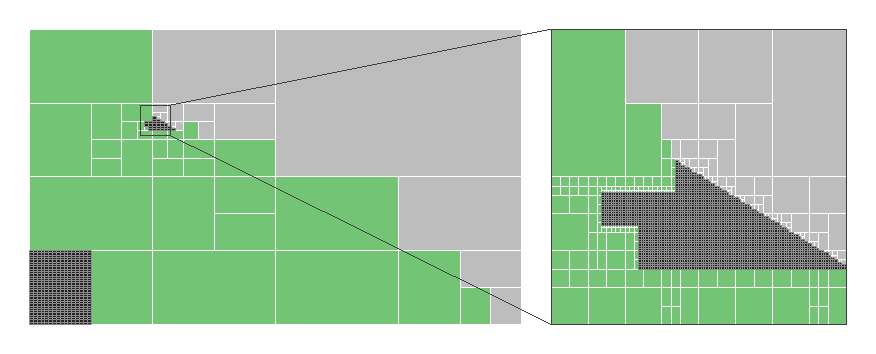
\includegraphics[width=\linewidth]{figures/exotic-directions}
\caption{The plane $\mathbf r=\mathbf 0$ of aligned configurations, with $s\in[0,2/3]$ horizontally and $t\in[0,2/5]$ vertically, halved $14$ times with the \fc{Domain}{Domain (grey)}, Global and \fc{Local}{Local (green)} components; right, the window of half-width $1/48$ around the point where the edge-on line $s=(\varphi-1)t$ meets the long side of the viewing triangle. Every configuration of this plane is a touch configuration, so the Global component eliminates none of it: beyond the viewing triangle the Domain component removes it, and inside only the Local covers eliminate pieces. They reach every viewing direction of the triangle except those near the corner $(0,0)$ and near that point, where the pieces stay unresolved (black) at any depth.}
\label{fig:exotic-directions}
\end{figure}
